\hypertarget{component-experiments}{\subsection{Targeted evaluations}}
\label{sec:component-specific}

\begin{figure}
\centering
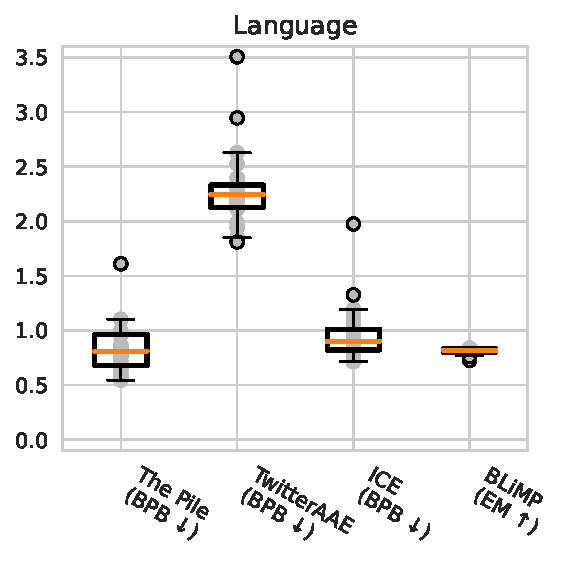
\includegraphics[width=.4\textwidth]{plots/component_language.pdf}
  \caption{\textbf{Targeted evaluation of language.
  Model accuracy on the four scenarios for evaluating linguistic understanding.
  } 
  }
  \label{fig:component-language}
\end{figure}

\paragraph{Language.} 
To further explore the results for this targeted evaluation, see \benchmarkUrlPrefix{language} and \reffig{component-language}.
For the language modeling scenarios, we begin by noting that the models trained on \pile are consistently the most accurate on \pile to no surprise.
However, these models also tend to be the most accurate on the other two language modeling scenarios: for \twitteraae and \ice, the most accurate models are \gptj, \gptneox, \optsixsix, \optonesevenfive, and \bloom. 
This suggests that \pile, when compared with the other training sets for these models, may yield better transfer to other language modeling datasets.
Further, we are surprised to see the other models trained on \pile, especially \anthropic and \mtnlgfivethreezero, which are generally are the most accurate models on the \core scenarios (\reffig{head-to-head}), are actually less accurate on \twitteraae and \ice compared to models not trained on \pile.
Overall, we see that the models that perform most accurately on all language modeling scenarios are quite different and are poorly correlated with the accuracy trends for \core scenarios.

Further, since \twitteraae and \ice provide unique demographic data, we examine performance disparities for these scenarios.
For \twitteraae, we see a clear and consistent trend: all models perform noticeably worse on the African American English subset when compared with the White English subset.\footnote{See \benchmarkUrlPrefix{twitter_aae}.} 
Consistent with prior work  on other language technologies \citep{blodgett2017racial, koenecke2020racial}, this indicates a clear performance disparity between language model performance for African American speakers vs. White speakers along the lines of historical marginalization.
All models for the Black subset have BPB above 2.0 (lower is better), whereas almost all models for the White subset are below 1.9, with the best model of \optonesevenfive having a BPB of 1.506 for the White English subset and 2.114 for the AAE subset.
For \ice, across all four regional subsets (East Africa, Hong Kong, India, USA), the most accurate models are the same as those mentioned above for \ice and the other language modeling scenarios overall.\footnote{See \benchmarkUrlPrefix{ice}.}
Further, we see the accuracies for the USA and East Africa tend to be better across all models, with EA being slightly worse, and then India and Hong Kong are clearly worse. 
For binary gender, we find that the female subset is consistently, but slightly, worse for model accuracy compare to the male subset.

Turning to \blimp, we find that all models achieve similar accuracies.
In fact, even on specific subsets for specific linguistic phenomena, we see the accuracies are quite similar. 
We are surprised to see \instructdavinci is not one of the most accurate models overall and, instead, is one of the least accurate models on the irregular forms (morphology) and quantifiers (semantics) subsets. 
Given its consistently high accuracies on various downstream tasks, this may indicate either a con of instruction-tuning or an over-generalization of linguistic rules, especially given the poor performance is on irregular forms in particular. 

\begin{figure}
\centering
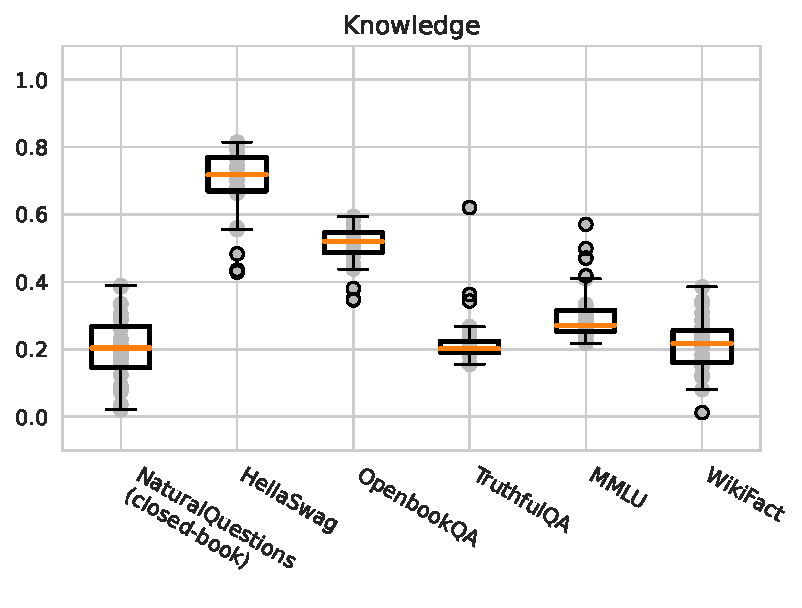
\includegraphics[width=.6\textwidth]{plots/component_knowledge.pdf}
  \caption{\textbf{Targeted evaluation of knowledge.}   
  Model accuracy on the six scenarios (5 question answering, \wikifact) for evaluating knowledge acquisition.
  }
  \label{fig:component-knowledge}
\end{figure}

\paragraph{Knowledge.}
To further explore the results for this targeted evaluation, see \benchmarkUrlPrefix{knowledge} and \reffig{component-knowledge}.
Across all five knowledge-intensive QA scenarios, we see \instructdavinci is the most accurate.
In particular, the gap in accuracies is especially salient for \truthfulqa, where \instructdavinci has an accuracy of 62.0\% and the next most accurate model is \anthropic at 36.2\% and for \mmlu, where \instructdavinci has an accuracy of 57.0\% and the next most acccurate model is \anthropic at 49.8\%. 
Of these scenarios, for the two that are more centric on factual knowledge (\ie \mmlu and \naturalquestions (closed-book)), we see that \mtnlgfivethreezero performs notably well, achieving an accuracy within 0.5\% of \instructdavinci for \naturalquestions (closed-book). 
This aligns clearly with the broader hypothesis that model scale is especially beneficial for memorizing specific factual information, which in turns proves useful for these very knowledge-intensive evaluations. 

To further hone in on specific factual knowledge, we then consider model accuracies on \wikifact.\footnote{See \benchmarkUrlPrefix{wikifact}.} 
We again see that \instructdavinci is the most accurate at 38.5\%, with \mtnlgfivethreezero as the second most accurate at 34.3\%, and with \coherexl (33.4\%) and \gptdavinci (39.7\% as the only other models above 30\%. 
For specific subsets we see more variation: for the \textit{plaintiff} relation type, all of \instructdavinci, \mtnlgfivethreezero and \coherexl are above 60\%, with the next best model being \jurassicjumbo at 51.0\% and \gptdavinci being considerably worse (46.5\%) despite its overall high accuracy. 
With that said, in spite of its significantly larger model size, there is no subset where \mtnlgfivethreezero performs significantly more accurately than all other models.
And all models perform quite poorly for some subsets, \eg the most accurate model gets an accuracy below 15\% for the \textit{discoverer\_or\_inventor} relation type.

\begin{figure}
\centering
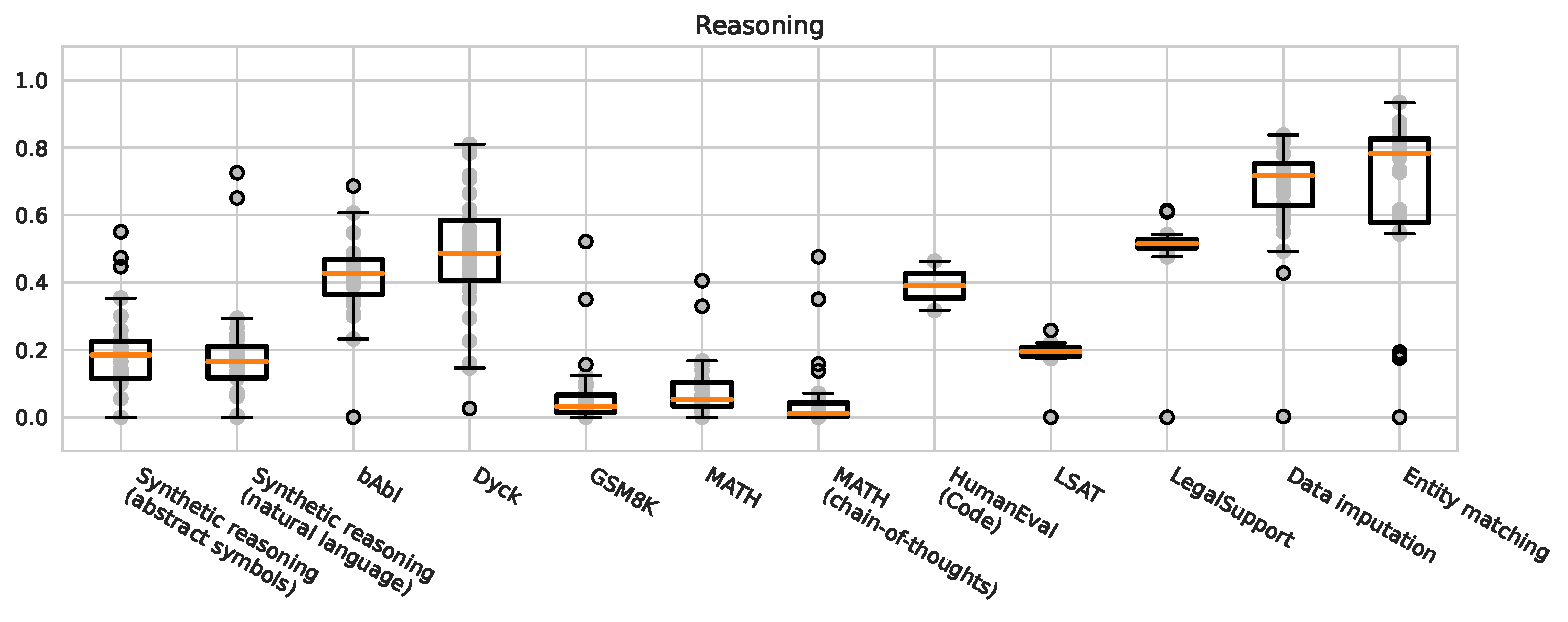
\includegraphics[width=\textwidth]{plots/component_reasoning.pdf}
  \caption{\textbf{Targeted evaluation of reasoning.}   
  Model accuracy on 12 scenarios (5 question answering, \wikifact) for evaluating reasoning capabilities.
  }
  \label{fig:component-reasoning}
\end{figure}

\paragraph{Reasoning.}
To further explore the results for this targeted evaluation, see \benchmarkUrlPrefix{reasoning} and \reffig{component-reasoning}.
Models are most accurate for the structured-data tasks such as entity matching and data imputation \citep{narayan2022can}, which are primarily based on pattern matching and classification.
In contrast, models are relatively inaccurate for tasks that involve abstraction, transitive inference, algebraic and logical reasoning, with natural-language tasks such as \lsat \citep{zhong2021arlsat} and \gsm \citep{cobbe2020leveraging} yielding low accuracies.
Overall, we find \davincicodex is consistently the most accurate model across reasoning scenarios, even in spite of some scenarios being posed fully in natural language. 

For both synthetic reasoning scenarios, we see no model achieves an accuracy above 40\% with the exception of \instructdavinci (47.3\% on abstract symbols, 65.1\% on natural language) and \davincicodex (55.0\% on abstract symbols, 67.3\% on natural language). 
That is, these two models show a clear and significant advantage in accuracy for these scenarios, with the gap between them shrinking in the presence of natural language while still maintaining that \davincicodex is more accurate than \instructdavinci for reasoning. 
We observe that similar trends hold for \MATH, \gsm, \babi, and \MATH (chain-of-thoughts). 
Looking at individual subsets for \babi, we find tasks 3, 4, 15 and 19, which assess transitive reasoning, relational understanding, deduction and planning skills, respectively, to be the the most challenging.\footnote{See \benchmarkUrlPrefix{babi_qa}.}
In contrast to the trends for \instructdavinci, for Dyck, we observe that \instructdavinci is not quite accurate (59.4\% accuracy), whereas \mtnlgfivethreezero (78.4\%) joins \davincicodex (80.2\%) as the only models above 75\%. 

For \lsat \citep{zhong2021arlsat}, which consists of reasoning questions posed for law school admissions, we observe that most evaluated models perform poorly, with accuracies around chance level (20\%). 
Looking into the behavior for individual examples, we see significant variation in behavior that is likely indicative of the spectrum of difficulty of questions.
On code scenarios, we see consistent trends with \davincicodex consistently outperforming \cushmancodex for both \humaneval and \codeapps, sometimes by large margins (\eg 10.\% strict correctness vs. 2.6\% on \codeapps). 
We note that we do not evaluate any of text models on these code scenarios, though in some cases this may be sensible/desirable given the striking generality of model development, deployment, and validation/scrutiny. 
Conversely, while we evaluate the code models for \lsat and \legalsupport, we find achieve accuracies of 0\%. 
Overall, we find \instructdavinci and, especially, \davincicodex display very strong reasoning capabilities for many different forms of reasoning. 

%%% Shorter version:
% For the LSAT task in particular \citep[\lsat;][]{zhong2021arlsat} which consists of law school reasoning questions, we see that most evaluated models perform poorly, obtaining results around chance level (20\%,), with a large performance variance between particular questions, indicating a range of difficulty degrees among questions. Providing models with rationales for selected in-context examples indeed reveals how the model's reported reasoning process is often logically flawed, lacking factual support, self-contradictory or even nonsensical.

%%% Longer version:
% Meanwhile, for the natural-language LSAT task \citep[\lsat;][]{zhong2021arlsat}, which consists of genuine Law School Admissions Tests given to prospective students, most evaluated models perform poorly, obtaining results around or below chance level of 20\%, regardless of the model size or the question type. There are some exceptions on specific question types, where for instance OpenAI-Davinci achieves 25.8\% on assignment questions and A21-Grande achieves 27.8\% on grouping questions, but we do not observe a consistent or significant trend. We also observe a large variance between performance on different examples, where for some particular questions most models achieve the right answer, while for other ones most models are mistaken, indicating a varied degree of difficulty among questions.

% To further study the behavior of models on this task, we have performed an additional small-scale exploratory experiment where as part of the input in-context prompt, we provide rationales for the reasoning process necessary to resolve the questions, and then ask the evaluated model to produce rationales for new examples. We inspected a few of the results, which reveal that models generate rationales that match in the writing style but are logically flawed (``By condition 1, A is located after B'' when the first condition in the question does not specify that), self-contradictory (``A must go first and therefore the answer is 2: A goes second''), making leaps of reasoning (``A plays after B, and B plays 2nd, therefore A must play 5th''), refer to non-existent supporting statements in the question (``By conditions 5 and 6...'' where there are only 4 conditions), or in the worst case are completely nonsensical (``By conditions 2, 3, or 5 by elimination, N is reduced, and therefore, by condition 1, W is eliminated as well. Therefore 2 is eliminated as well.'', referring to irrelevant conditions and mixing elimination of letters which refer to items and numbers which refer to conditions).

\begin{figure}
\centering
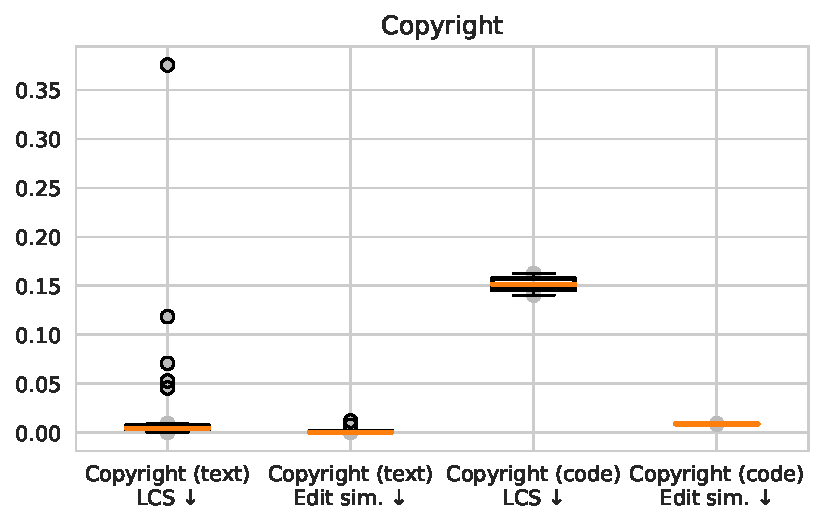
\includegraphics[width=0.75\textwidth]{plots/copyright.pdf}
% 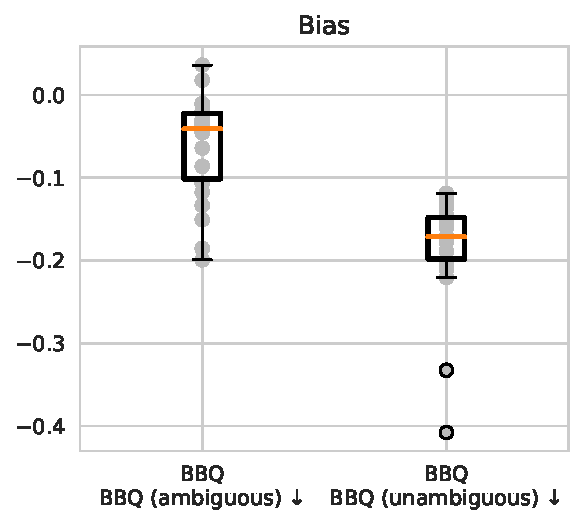
\includegraphics[height=.29\textwidth]{plots/bias.pdf}
% 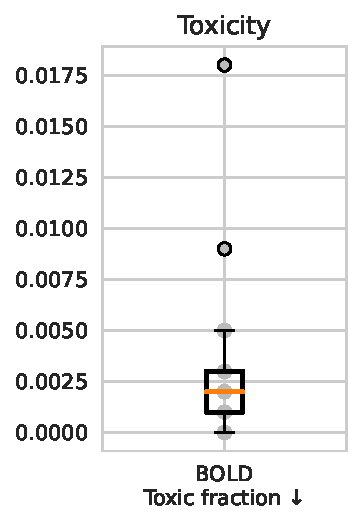
\includegraphics[height=.29\textwidth]{plots/toxicity.pdf}
  \caption{\textbf{Targeted evaluation of copyright and memorization.} 
  Model performance on targeted evaluations for memorization for both copyrighted text and licensed code. 
  }
  \label{fig:component-copyright}
\end{figure}

\begin{figure}
\centering
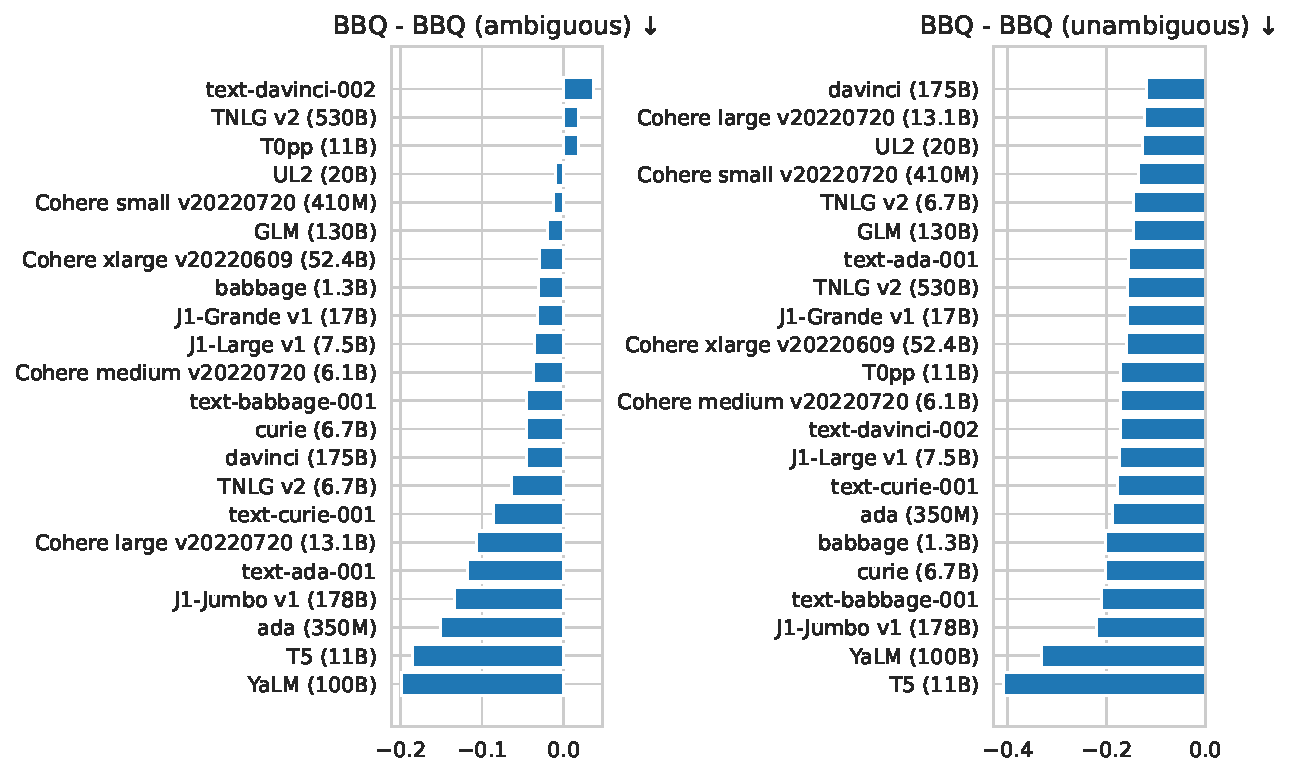
\includegraphics[width=0.75\textwidth]{plots/bias_bars.pdf}
%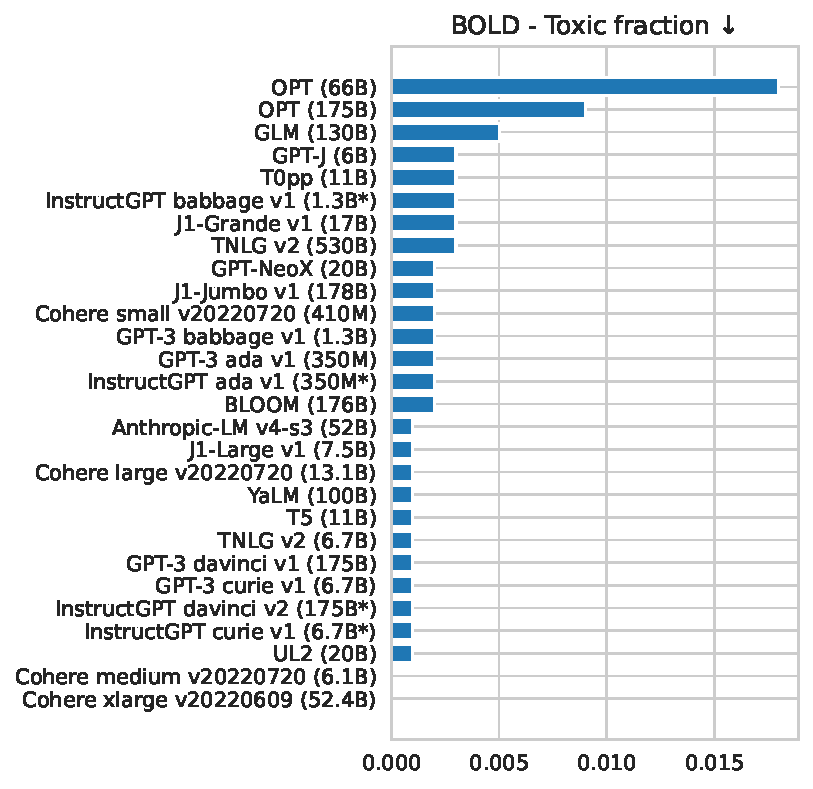
\includegraphics[height=.5\textwidth]{plots/toxicity_bars.pdf}
  \caption{\textbf{Targeted evaluation of social bias.} 
  Model performance on targeted evaluations for bias on \bbq. 
  }
  \label{fig:component-bias}
\end{figure}

\paragraph{Memorization \& Copyright.}
To further explore the results for this targeted evaluation, see \benchmarkUrlPrefix{copyright_text}, \benchmarkUrlPrefix{copyright_code} and \reffig{component-copyright}.
We evaluated various models for their ability to reproduce copyrighted text or licensed code. 
When evaluating source code regurgitation, we only extract from models specialized to code (\davincicodex and \cushmancodex).
When evaluating text regurgitation, we extract from all models except those specialized to code. 

Overall, we find that models only regurgitate infrequently, with most models not regurgitating at all under our evaluation setup. 
However, in the rare occasion where models regurgitate, large spans of verbatim content are reproduced. 
For instance, while no model in our suite reliably reproduces content given prompts taken from randomly sampled books, some models can reproduce large chunks of popular books given short prompts.
Notably, we observe that \gptdavinci and \anthropic reproduce non-trivial spans of the first few pages of several Harry Potter books, and \optonesevenfive and \anthropic reproduce large spans of the children's book ``Oh, the Places You'll Go!''
% \footnote{
% \url{https://crfm.stanford.edu/helm/v0.1.0/?group=copyright_text&subgroup=datatag\%3A\%20popular_books-prefix_length_125.json\#Copyright\%20(text)}
% }

On average, we see that models specialized to code reproduce source code content to a larger degree than non-code models for text with the prompt sources we collected (\eg \reffig{component-copyright} shows that both the prefix-length-normalized LCS and edit similarity are higher for the code component than the text component). 
In addition, we observe cases where the code model not only reproduces the functional aspects of the code but also the comments verbatim.

\paragraph{Disinformation.}
Since we do not have automated metrics at present for many aspects of human evaluation, and the effectiveness of disinformation strongly depends on (potentially very) subjective human judgments, we primarily measure model behavior for disinformation through human evaluation.
Consequently, we defer discussion to \refsec{human-evaluation-disinformation}. 

\paragraph{Bias.}
To further explore the results for this targeted evaluation, see \benchmarkUrlPrefix{bbq}.
For \bbq, we begin by noting the very striking finding for model accuracy: \instructdavinci achieves an accuracy of 89.5\%, which is much greater than any other model, with \tzero (48.4\%) and \mtnlgfivethreezero (44.9\%) as the second and third most accurate, with not other model achieving accuracy above 40\%.

With this in mind, we see that accuracy shows a very strong clear correlation with social bias in ambiguous contexts (\reffig{component-bias}).
That is, \instructdavinci demonstrates the strongest bias that aligns with overarching societal biases and marginalization in ambiguous contexts, and the other two models are the only other ones with similar biases.
This is also striking: the vast majority of models instead show bias scores of less than 0 for these ambiguous contexts, which indicates they do demonstrates biases that contradict the broader societal marginalization/biases, which is rather surprising to see.

Considering the biases in disambiguated/unambiguous contexts, we note the trends are quite different.
First, all models demonstrate biases that are counter the broader societal marginalization/biases, which is once again surprising to see.
Further, we see that the relationship between model accuracy on \bbq and bias in unambiguous contexts is much less clear: \instructdavinci, \tzero, and \mtnlgfivethreezero all are closer to the middle amidst the other models, rather than being at either extreme.
What we do see is that the \tfive and the \yalm models are the most strongly biases for both settings, both times in the same direction.
Further, noting that \tfive is the least accurate model for this scenario of all models, and \yalm is one of the less accurate models, we note this may suggest that the understanding of results for \bbq should take into account all three of these metrics to provide a fuller picture. 

\paragraph{Toxicity.}
To further explore the results for this targeted evaluation, see \benchmarkUrlPrefix{real_toxicity_prompts} and \benchmarkUrlPrefix{bold}.
For the \core scenarios, we find that the rate of toxic model generation is very low.
To the extent there is an exception, we see nontrivial toxicity generation for \narrativeqa, which is likely related to the contexts that situate and prime these generations (\ie stories).
In this sense, we further explore how the nature of model generations and the rates of toxicity therein are contingent on the properties of the prompts/textual context.

For both \realtoxicityprompts and \bolddataset, we consider the properties, namely toxicity, of model generations conditional on a distribution of prompts. 
In \realtoxicityprompts, \citet{gehman2020realtoxicityprompts} have already stratified the prompts based on whether they are toxic or not according to PerspectiveAPI.
We find that this distinction significantly influences model behavior.
For the toxic split, several models (\jurassicjumbo, \jurassiclarge, \jurassicgrande, \tzero, \gptdavinci, \instructdavinci, \instructcurie, \instructbabbage) all generate toxicity in at least 10\% of generations, with \yalm generating toxic in over 15\% of generations.
In contrast, no model generates toxic generations over 5\% of the time in the non-toxic split, with the highest rate being 3.4\% from \gptdavinci and the toxicity rate for \yalm dropping from 15.7\% to 2.8\%. 
These trends are even more salient on \bolddataset, where model generations for only 1 model (\optsixsix, 1.8\%) are toxic at least 1\% of the time. 
Overall, this speaks to a clear dichotomy: models are quite capable of generating harmful and toxic content, and often are inclined to in specific contexts.
But in many contexts encountered in deploying language models for legitimate use cases, we may find toxic generations to be quite rare (though it is worth emphasizing that even while rare, they can still have pronounced and acute social harms, perhaps even perpetuating prior harms to marginalized groups \citep{abid2021persistent}).  